% This file is iccc.tex.  It contains the formatting instructions for and acts as a template for submissions to ICCC.  It borrows liberally from the AAAI and IJCAI formats and instructions.  It uses the files iccc.sty, iccc.bst and iccc.bib, the first two of which also borrow liberally from the same sources.

\documentclass[letterpaper]{article}
\usepackage{iccc}


\usepackage{array,multirow}
%\newcommand{\bigcell}[2]{\begin{tabular}{@{}#1@{}}#2\end{tabular}}
\usepackage{hhline}% http://ctan.org/pkg/hhline
\usepackage{xcolor}

\usepackage{times}
\usepackage{helvet}
\usepackage{courier}

% Packages maison
\usepackage{amsmath,amssymb} % For including math equations, theorems, symbols, etc
\usepackage{bm}
\usepackage{graphicx} % Required for including images
\graphicspath{{../Figures/}} % Set the default folder for images
\usepackage{prettyref}

\pdfinfo{
/Title (Formatting Instructions for Authors)
/Subject (Proceedings of ICCC)
/Author (ICCC)}
% The file iccc.sty is the style file for ICCC proceedings.
%
\title{\textit{Live Orchestral Piano}, a system for real-time orchestral music generation}
\author{L\'eopold Crestel, Philippe Esling\\
\'Equipe Repr\'esentation Musicales\\
Institut de Recherche et Coordination Acoustique/Musique\\
1 Place Igor-Stravinsky, 75004 Paris\\
leopold.crestel@ircam.fr, philippe.esling@ircam.fr\\
}
\setcounter{secnumdepth}{0}

\begin{document} 
\maketitle
\begin{abstract}
\begin{quote}
This paper introduces the first system for performing automatic \textit{orchestration} based on a piano input. Our main hypothesis is that we can learn the underlying regularities existing between piano scores and their orchestrations by notorious composers, in order to automatically perform this task on novel piano inputs. To that end, we investigate a class of statistical inference models called \textit{conditional Restricted Boltzmann Machine} (\textit{cRBM}). We introduce a specific evaluation framework for orchestral generation based on a prediction task \textbf{in order to assess the quality of different models} \textbf{USEFULL TO PRECISE ?}. As prediction and creation are two widely different endeavours, we discuss the potential biases in evaluating generative models through prediction \textbf{3 TIMES PREDICTION IN 2 SENTENCES} tasks and their impact on a creative system. Finally, we introduce an implementation of the model \textbf{WHICH ONE ??} called \textit{Live Orchestral Piano} (LOP), which allows to perform real-time projective orchestration of \textbf{a MIDI keyboard input}.
\end{quote}
\end{abstract}

\section{Introduction}
% Orchestration classique
%% Musical orchestration : why is it so hard ?
% Orchestration
\textit{Orchestration} is the subtle art of writing musical pieces for the orchestra, by combining the properties of various instruments in order to achieve a particular sonic rendering. Because of its extensive reliance on spectral characteristics, orchestration is often referred to as the art of manipulating instrumental timbres \cite{mcadams2013timbre}. Timbre is defined as the property which allows to distinguish two sounds produced at the same pitch and intensity.
% -> Timbre
Hence, the sonic palette offered by the pitch range and intensities of one instrument is augmented by the wide range of expressive timbres produced through the use of different playing style.
\textbf{Hence, above the traditional harmonic and rhythmic structures, timbre becomes the most crucial dimension in orchestral works}\textbf{IT UNDERLINES IT NO, IS NOT MORE IMPORTANT ??}. Furthermore, it has been shown that some instrumental mixtures can not be expressed as a simple summation of their components, but can lead to a unique \textit{emerging timbre}, with phenomenon such as orchestral blend \cite{tardieu2012perception}.
% -> Combinatoire
Given the number of different instruments in a symphonic orchestra, their respective range of expressiveness (timbre, pitch and intensity), and the phenomenon of emerging timbre, one can foresee the extensive combinatorial complexity embedded in the process of orchestral composition.

Those difficulties have been a major obstacle towards the construction of a scientific basis for the study of orchestration. From a mathematical point of view, it seems that no set of descriptors can exhaustively fit with the perceptual complexity of timbre \cite{peeters2011timbre}. From a musical point of view, there is a lack of symbolic notation for timbre, and orchestration remains an empirical discipline taught through the observation of existing orchestration examples \cite{piston-orch}. Among the different techniques for writing orchestral pieces, one of them  consists in first writing an harmonic and rhythmic structure in the form of a piano score and then adding the timbre dimension by spreading the different voices over the various instruments \cite{piston-orch}. We refer to this operation of extending a piano draft to an orchestral score as \textit{projective orchestration} \cite{eslingthesis}.

\begin{figure}
\centering
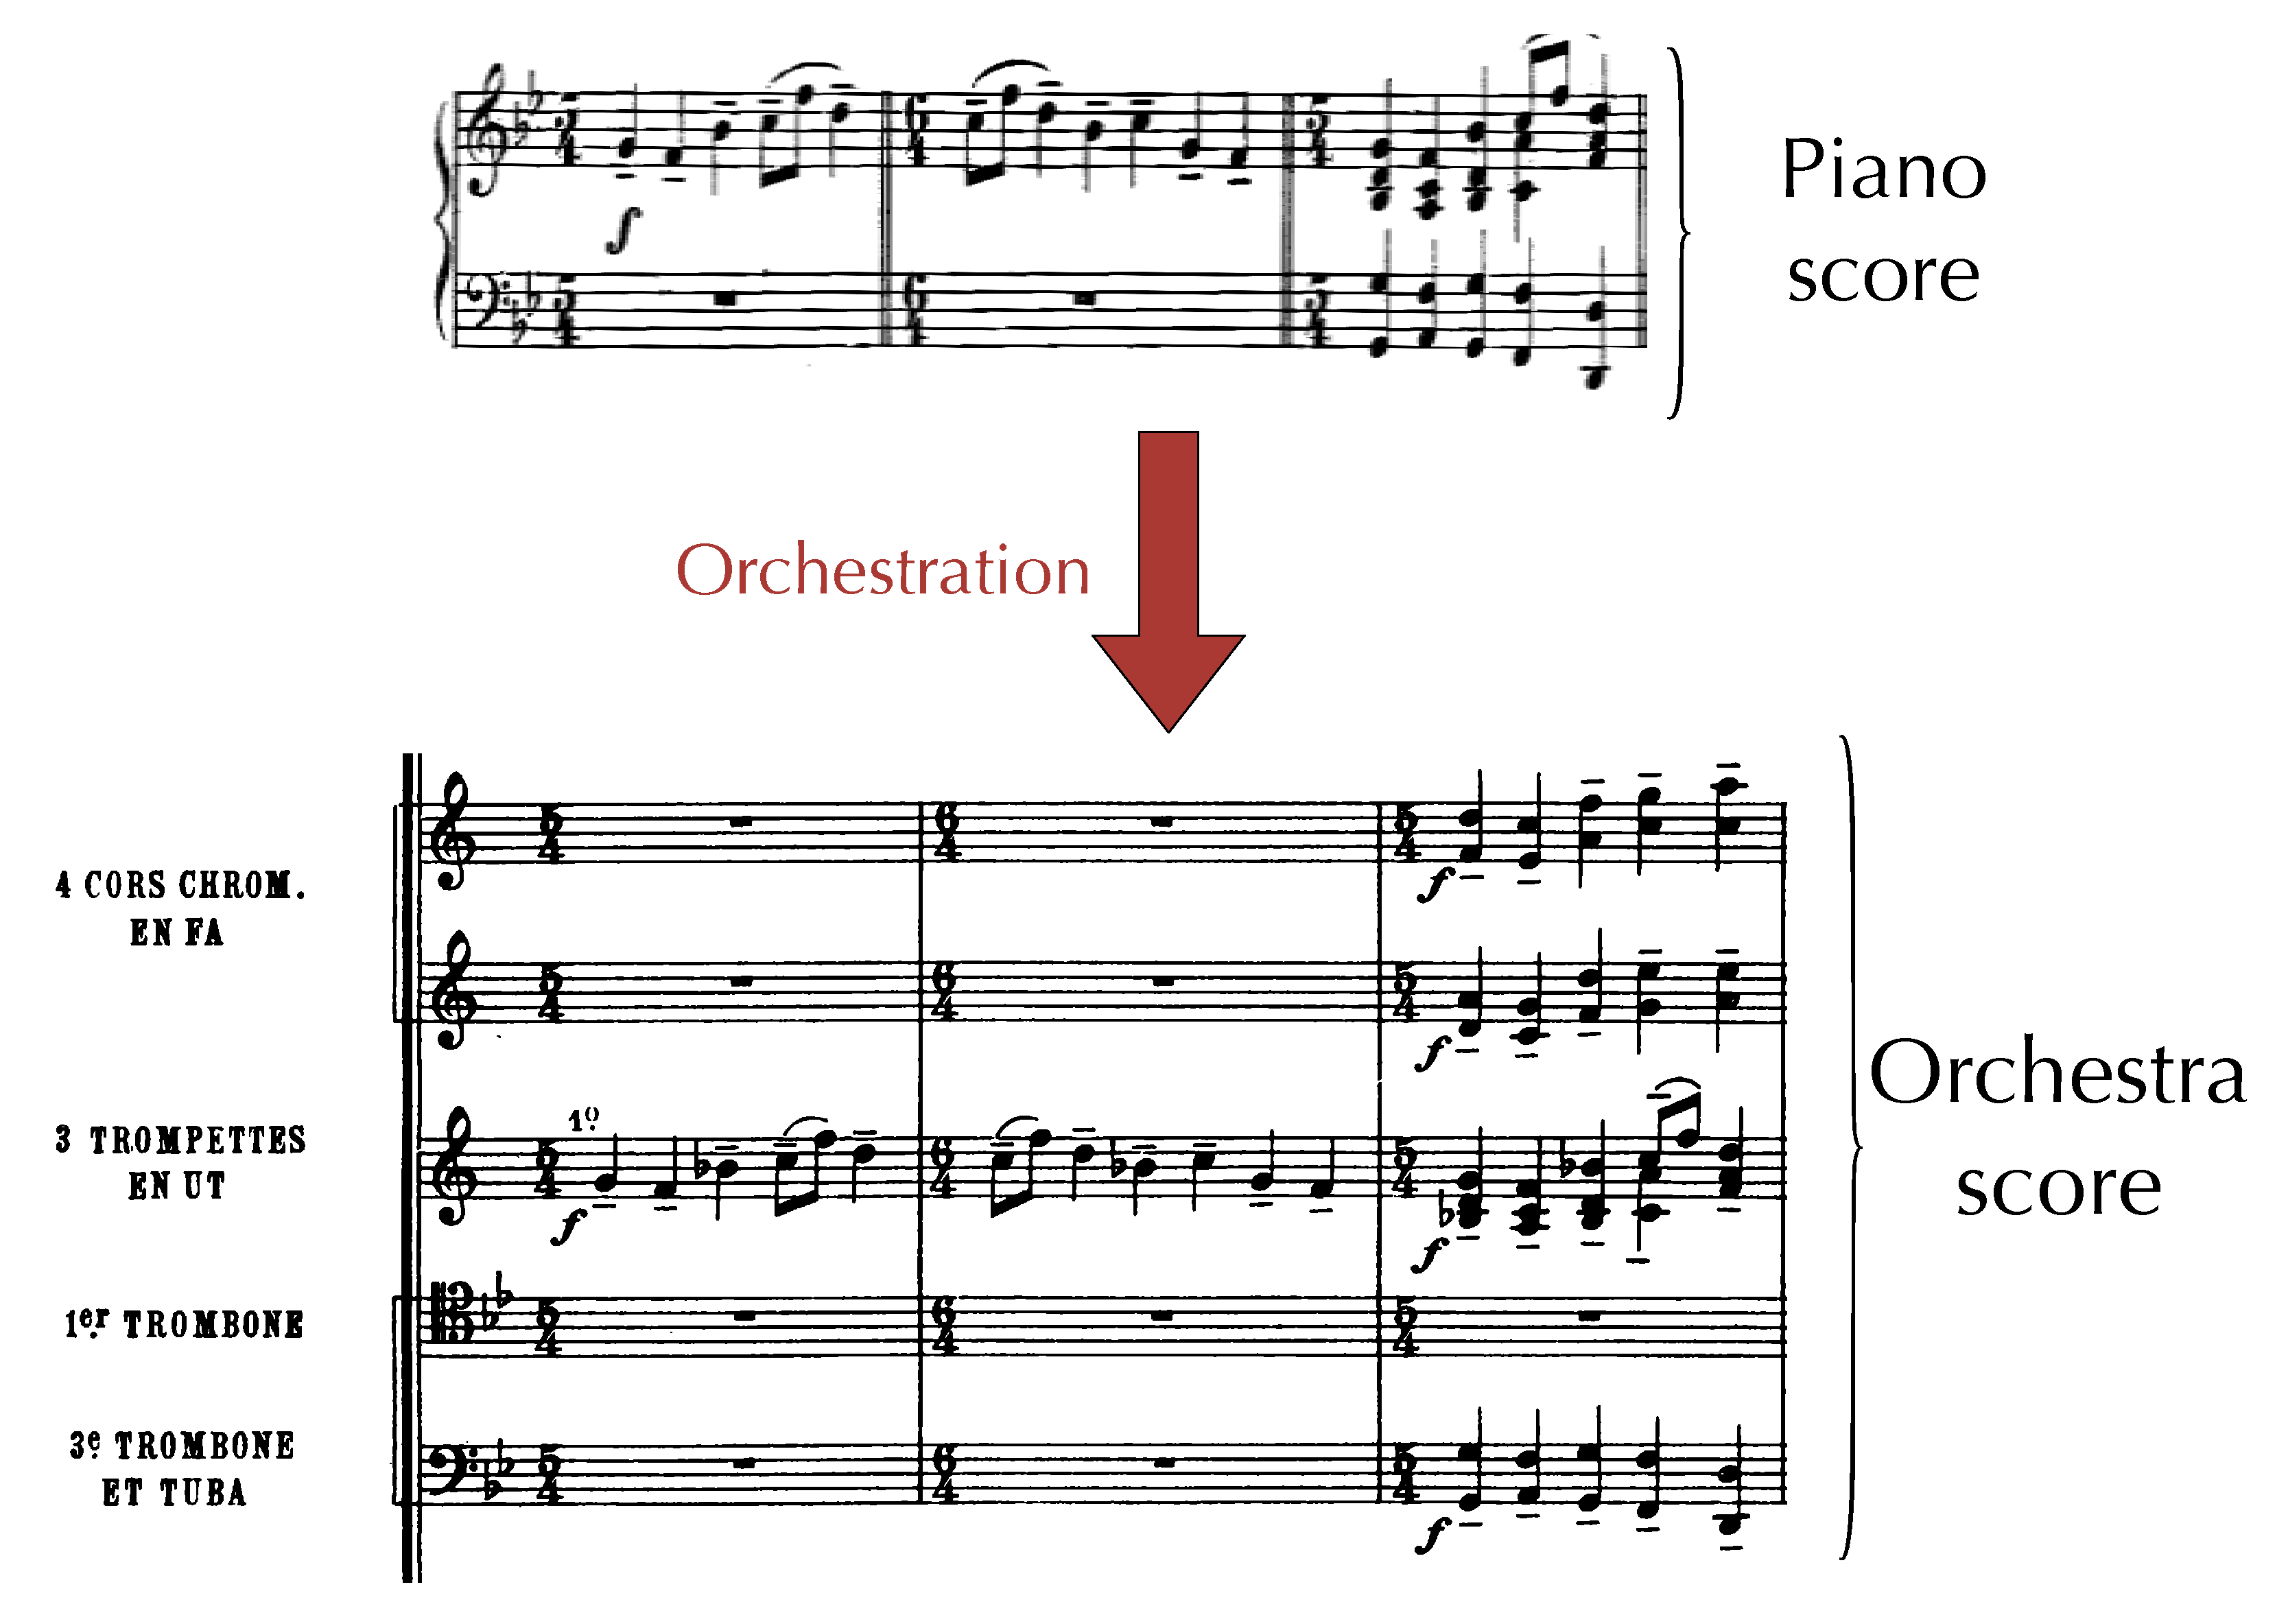
\includegraphics[scale=0.13]{orch}
\caption{\textit{Projective orchestration}. A piano score is projected on an orchestra. Even though for one piano score, a wide range of orchestrations exists, the relationships between a piano score and its orchestral realization implicitly embeds the knowledge of the composer about timbre.}
\label{fig:orch}
\end{figure}

The orchestral repertoire contains a large number of examples of projective orchestration (such as the piano reductions by Liszt of Beethoven symphonies or the \textit{pictures at an exhibition}, a piano piece by Moussorgsky orchestrated by several notorious composers). By observing a case of projective orchestration (see \prettyref{fig:orch}), we can clearly see that this process involves more than the mere allocation of notes written on the piano score across the different instruments. It rather imply harmonic densification \textbf{(REF)}, and timbre manipulations to underline the already existing harmonic and rhythmic structure \cite{mcadams2013timbre}. However, the visible correlations between a piano score and its orchestrations \textbf{appear as a || PROMISE A ??} fertile framework for laying the foundation of a computational exploration of orchestration. Even though systemic rules remain difficult to identify because of the high dimensionality of the problem and prevent us from building a general theory of orchestration, it does not mean that underlying local regularities could not be extracted.
\textbf{WHICH ONE ?????}
\textbf{Hence,  by attempting to unify under a same general description many particular cases could, in fact, lead to inferring a description of their inner structure sufficiently general to be able to generate novel examples.}
 \textbf{OR || Hence, defining partial rules to unify under a same general description many particular cases, could in turn be used to infer and generate novel examples.}

Statistical inference covers a range of methods for trying to automatically extract a structure from observations. These approaches hypothesize that a particular type of data might be structured by an underlying probability distribution. The objective is to deduce properties of this distribution, by observing a set of those data. A wide range of statistical inference models have been devised, among which deep learning recently appeared as a  promising field in artificial intelligence and representation learning \cite{bengio2013representation,LeCun:2015aa}. The building blocks of many models in this field is the \textit{Restricted Boltzmann Machine} (\textit{RBM}) \cite{hinton2006fast}. 


\textbf{Thus, our objective is to build a system of automatic projective orchestration. We believe that learning the underlying distribution of a corpus of piano score and their orchestration by famous composers through statistical inference is a promising lead toward the automatic generation of orchestrations with a sensible timbre structure/EVOLUTION ???}

In the context of projective orchestration, the data can be defined as the score, formed by a succession of pitch and intensities for each instrument. The set of observations would be the set of projective orchestrations performed by famous composers, and the probability distribution \textbf{would model the set of notes played by each instrument conditionally on a piano score.}

It might be surprising at first to rely solely on symbolic information (scores) whereas we insisted on the fact that orchestration is the art of timbre, typically not represented in the musical notation but rather conveyed in the signal information (audio recording). 
\textbf{However, we make the assumption that spectrally consistent orchestrations could be generated from a purely symbolic learning by uncovering the \textbf{composers' knowledge about timbre embedded in the score.} A LA PLACE DE : ||}
\textbf{However, we make the strong assumption that even though we work in a purely symbolic setting, as we rely on the work of composers that effectively took into account the resulting spectral effects, these symbolic relationships embed the spectral information.}

Hence, using statistical inference on a corpus linking piano scores to their projective orchestrations by famous composers could unveil part of timbre mixture properties of their orchestration techniques. \textbf{The specific approach of each composer would be assimilated by HZIUEHFIZUEF}

We focus on a class of models called \textit{Conditional RBM} \cite{taylor2006modeling}, which implements a notion of context particularly adapted to represent both the temporal dependencies in the orchestral score and the influence of the piano score.
Besides these structural advantages, those models are also generative, which means that once the underlying distribution of the observed data is correctly modelled, it is possible to generate orchestration from unseen piano scores.

To be able to select among different models, it is important to design a quantitative evaluation framework. Designing a criterion for the performance of a generative model is a major pitfall (\textbf{REF???}). In the polyphonic music generation field, a predictive task is commonly used \cite{DBLP:journals/corr/YaoCVDD15,boulanger2012modeling,lavrenko2003polyphonic}. Relying on these works, we introduce a specific framework for projective orchestration and discuss the results of the \textit{cRBM} and \textit{FGcRBM} models.

Finally, an interesting property of both \textit{cRBM} and \textit{FGcRBM} models is their ability to generate orchestration from an unseen piano score sufficiently fast for a real-time implementation.
Using the defined performance criterion we selected the most efficient model and implemented it in a system called \textit{Live Orchestral Piano} (LOP), a real-time orchestration interface from a piano input.

The remainder of this paper is organized as follows. The first section introduces the state of the art in conditional models, in which RBM, cRBM and \textit{FGcRBM} models are detailed. The projective orchestration task is presented in the next section along with an evaluation framework based on a frame-level accuracy measure. The introduced models are evaluated within this framework and compared to existing models. Then, we introduce \textit{LOP}, the real-time projective orchestration system. Finaly, we provide our conclusions and directions of future work.

\section{State of the art}
\label{sec:state_of_the_art}
In this section, three statistical inference models are detailed. The \textit{RBM}, \textit{cRBM} and \textit{FGcRBM} are presented by increasing level of complexity, each model adding a new \textit{degree of freedom} to the previous one.

\subsection{Restricted-Boltzmann Machine}
The \textit{RBM} \cite{hinton2006fast} is a graphical probabilistic model (\prettyref{fig:RBM}) composed by a set of $I$ visible units $\bm{v} = (v_{1},...,v_{I})$, each representing a binary random variable. Note that this model can be extended to continuous variables \cite{hinton2010practical}. Despite this is not a general truth, those visible units usually model the observed data in which case $I$ is equal to the dimension of those data. An other set of $J$ binary random variables ($\bm{h} = (h_{1},...,h_{J})$) are called hidden (or latent) units. They are connected to visible units through weights $W_{ij}$ which model conditional dependencies between visible and hidden units through the relations
\begin{align}
\label{eq:marginal_RBM_1}
p(h_{j}=1|\bm{v}) &= \sigma \left( b_{j} + \sum_{i}W_{ij}v_{i} \right)
\end{align}
\begin{align}
\label{eq:marginal_RBM_2}
p(v_{i}=1|\bm{h}) &= \sigma \left( a_{i} + \sum_{j}W_{ij}h_{j} \right)\\
\end{align}
where $\sigma	(x) = \frac{1}{1+e^{-x}}$ is the \textit{sigmoid} function . The biases $a_{i}$ and $b_{j}$ act as a permanent offset to the activation of a unit. Along with weights, they form parameters of the model $\bm{\theta} = \left\lbrace \bm{W} , \bm{a} , \bm{b} \right\rbrace$

The joint probability of the visible and hidden random variables is given by $p_{model}(\bm{v},\bm{h}) = \frac{\exp^{-E(\bm{v},\bm{h})}}{Z}$ where
\begin{equation}
\label{eq:energy}
E(\bm{v},\bm{h}) = - \sum_{i=1}^{m} a_{i} v_{i}  - \sum_{i=1}^{m} \sum_{j=1}^{n} v_{i} W_{ij} h_{j} - \sum_{j = 1}^{n} b_{j} h_{j}
\end{equation}
is the energy function associated to the model. $Z = \sum_{v,h}\exp^{-E(v,h)}$ is a normalizing factor called partition function which ensures that the sum of the probabilities over the possible configuration of visible and hidden variables is equal to one.

Training a model on a set of data means that we want the distribution of the model ($p_{model}$) to be as close as possible to the hypothetical distribution of the data ($q_{data}$).
A commonly used criterion for training this model is to maximize the likelihood of the training set, which can be interpreted as the probability that the observed data have been generated by the model.
The vectors from the training set $\mathcal{D}$ are designated by $\bm{v^{(l)}}$.
Instead of maximizing the likelihood, minimizing the negative log-likelihood is often preferred as it simplifies the mathematical expressions
\begin{equation}
\label{eq:likelihood}
\mathcal{L(\bm{\theta}|\mathcal{D})}  = \frac{1}{N_{\mathcal{D}}} \sum_{\bm{v^{(l)}} \in \mathcal{D}} - \ln \left( p(\bm{v^{(l)}}|\bm{\theta})\right)
\end{equation}
where $N_{\mathcal{D}}$ is the size of the dataset. 

The search for the minimum of this non-linear function can be tackled by using gradient descent \cite{bottou2010large}. The gradient of the negative log-likelihood of any vector from the training database $\bm{v}^{(l)}$ is given by
\begin{equation}
\label{eq:loglik}
\begin{split}
- \frac{\partial \ln \left[ p(\bm{v^{(l)}}|\bm{\theta})\right]}{\partial \bm{\theta}} 
= 
\mathbb{E}_{p(\bm{h}|\bm{v^{(l)}})} \left[ \frac{\partial E(\bm{v^{(l)}},\bm{h})}{\partial \bm{\theta}} \right] 
- \\
\mathbb{E}_{p(\bm{v} , \bm{h})} \left[ \frac{\partial E(\bm{v},\bm{h})}{\partial \bm{\theta}} \right]
\end{split}
\end{equation}
It is interesting to note that this represents the difference between two expectations of the same quantity. The first left-side expectation is referred to as the \textit{data-driven} term since it is an expectation over the distribution of the hidden units conditionally on a specific sample from the data distribution. The expectation on the right is referred to as the \textit{model-driven} term since it is an expectation over the joint distribution of the model.
Unfortunately the model-driven quantity is intractable because it involves a sum over all the possible configurations of the hidden (alternatively visible) units in order to compute the partition function \cite{Fischer2012}.

In order to alleviate this problem, a training algorithm called Contrastive Divergence (\textit{CD}) \cite{hinton2002training} proposes to approximate the model driven term by
\begin{equation}
\label{eq:grad_log_like}
\begin{split}
- \frac{\partial \ln \left[ p(\bm{v^{(l)}}|\bm{\theta})\right]}{\partial \bm{\theta}}
\approx 
\mathbb{E}_{p(\bm{h}|\bm{v^{(l)}})} \left[ \frac{\partial E(\bm{v^{(l)}},\bm{h})}{\partial \bm{\theta}} \right] 
- \\
\mathbb{E}_{p(\bm{h} | \bm{v^{(l,k)}})} \left[ \frac{\partial E(\bm{v^{(l,k)}},\bm{h})}{\partial \bm{\theta}} \right]
\end{split}
\end{equation}
where $\bm{v}^{(l,k)}$ is obtained by running a k-step Gibbs chain. A Gibbs chain consists in alternatively sampling the hidden units knowing the visible units (\prettyref{eq:marginal_RBM_1}) and the visible knowing the hidden \prettyref{eq:marginal_RBM_2}.

Note that sampling from the marginal distribution is easy since visible units (respectively hidden units) are independent from each others. Hence, knowing the hidden units, all the visible units can be sampled in one step. This allows for a fast implementation of the sampling step through matrix calculus, known as \textit{block sampling}.
It has been proved \cite{bengio2009learning} that the samples obtained after an infinite number of iterations will be drawn from the joint distribution of the visible and hidden units of the model. Approximations in running the Gibbs chain can be made by starting the chain from the same sample $\bm{v}^{(l)}$ used in the \textit{data-driven} term. This speed-up the convergence of the chain. A second approximation is to limit the number of sampling steps to a fixed number K. After evaluating the statistics of the distribution $\bm{h} \sim p(\bm{h}|\bm{v^{(l)}})$ and $\bm{v^{(l,k)}}$ and $\bm{h}\sim p(\bm{h}|\bm{v^{(l,k)}})$ from the Gibbs sampling chain, the parameters can be updated. By introducing the notation $<>_{data}$ (respectively $<>_{model}$) to express an expectation over the data (respectively model) distribution the update rules in a \textit{RBM} are given by
%%% En fait, si on est rigoureux, <> c'est p(h|v)_model ou data et dans le deuxième c'est v^(K)...
\begin{align}
\Delta W_{ij} &= <v_{i}h_{j} >_{data} - <v_{i}h_{j} >_{model}\\
\Delta a_{i} &= <v_{i}>_{data} - <v_{i}>_{model}\\
\Delta b_{j} &= <h_{j} >_{data} - <h_{j} >_{model}
\end{align}
\begin{figure}
\centering
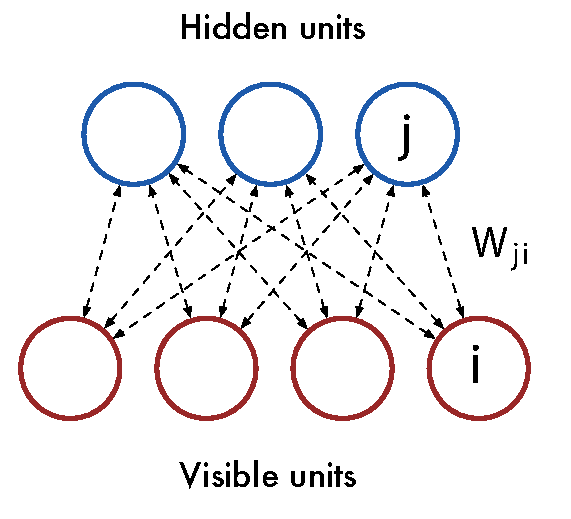
\includegraphics[scale=0.7]{RBM}
\caption{The \textit{Restricted Boltzmann Machine} (RBM) is defined by a set of visible ($v_{i}$)) and hidden ( $h_{j}$) units.  Symmetric weights ($W_{ij}$) connect a hidden unit to a visible unit which altogether define an energy function $E_{W}(v,h)$. Training an \textit{RBM} consists in modifying the weights $W$ to lower the energy function for the points observed in the training set.}
\label{fig:RBM}
\end{figure}

\subsection{Conditional RBM}
The conditional \textit{RBM} (\textit{cRBM}) model \cite{taylor2009factored} is an extension of the \textit{RBM} in which dynamic biases are added to the biases of the visible ($\bm{a}$) and hidden ($\bm{b}$) units. These dynamic biases linearly depend on a set of $K$ context units denoted $\bm{x} = (x_{1},...,x_{K})$. In the case of time series, if the visible units represent a frame at time $t$, these context units can be used to model the influence of the recent past frames $\left[ t-N, t-1 \right]$ on the current frame ($N$ defining the \textit{temporal order}).
Thus the energy function of the \textit{cRBM} is given by
\begin{equation}
\begin{split}
\label{eq:energy_cRBM}
E(\bm{v}(t),\bm{h}(t)|\bm{x}(t)) =  - \sum_{i} \hat{a}_{i}(t)v_{i}(t) - \\ \sum_{ij}W_{ij}v_{i}(t)h_{j}(t) - \sum_{j} \hat{b}_{j}(t)h_{j}(t)
\end{split}
\end{equation}
where the biases are defined by 
\begin{align*}
\hat{a}_{i}(t) &= a_{i} + \sum_{k}A_{ki}x_{k}(t)\\
\hat{b}_{j}(t) &= b_{j} + \sum_{k}B_{kj}x_{k}(t)
\end{align*}
We will refer to the matrices $\bm{A}$ and $\bm{B}$ as \textit{auto-regressive matrices}.

This model can be trained using CD, since the marginal probabilities of visible and hidden units are the same as the \textit{RBM} (simply replacing the static biases by dynamics ones).
Hence, the update rules are unchanged for $\bm{W}$, $\bm{a}$ and $\bm{b}$, and are given for the auto-regressive matrices by
\begin{align}
\Delta A_{ik} 	&=<v_{i}x_{k} >_{data} - <v_{i}x_{k} >_{model}\\
\Delta B_{jk} 	&= <h_{j}x_{k} >_{data} - <h_{j}x_{k} >_{model}\\
\end{align}

\begin{figure}
\centering
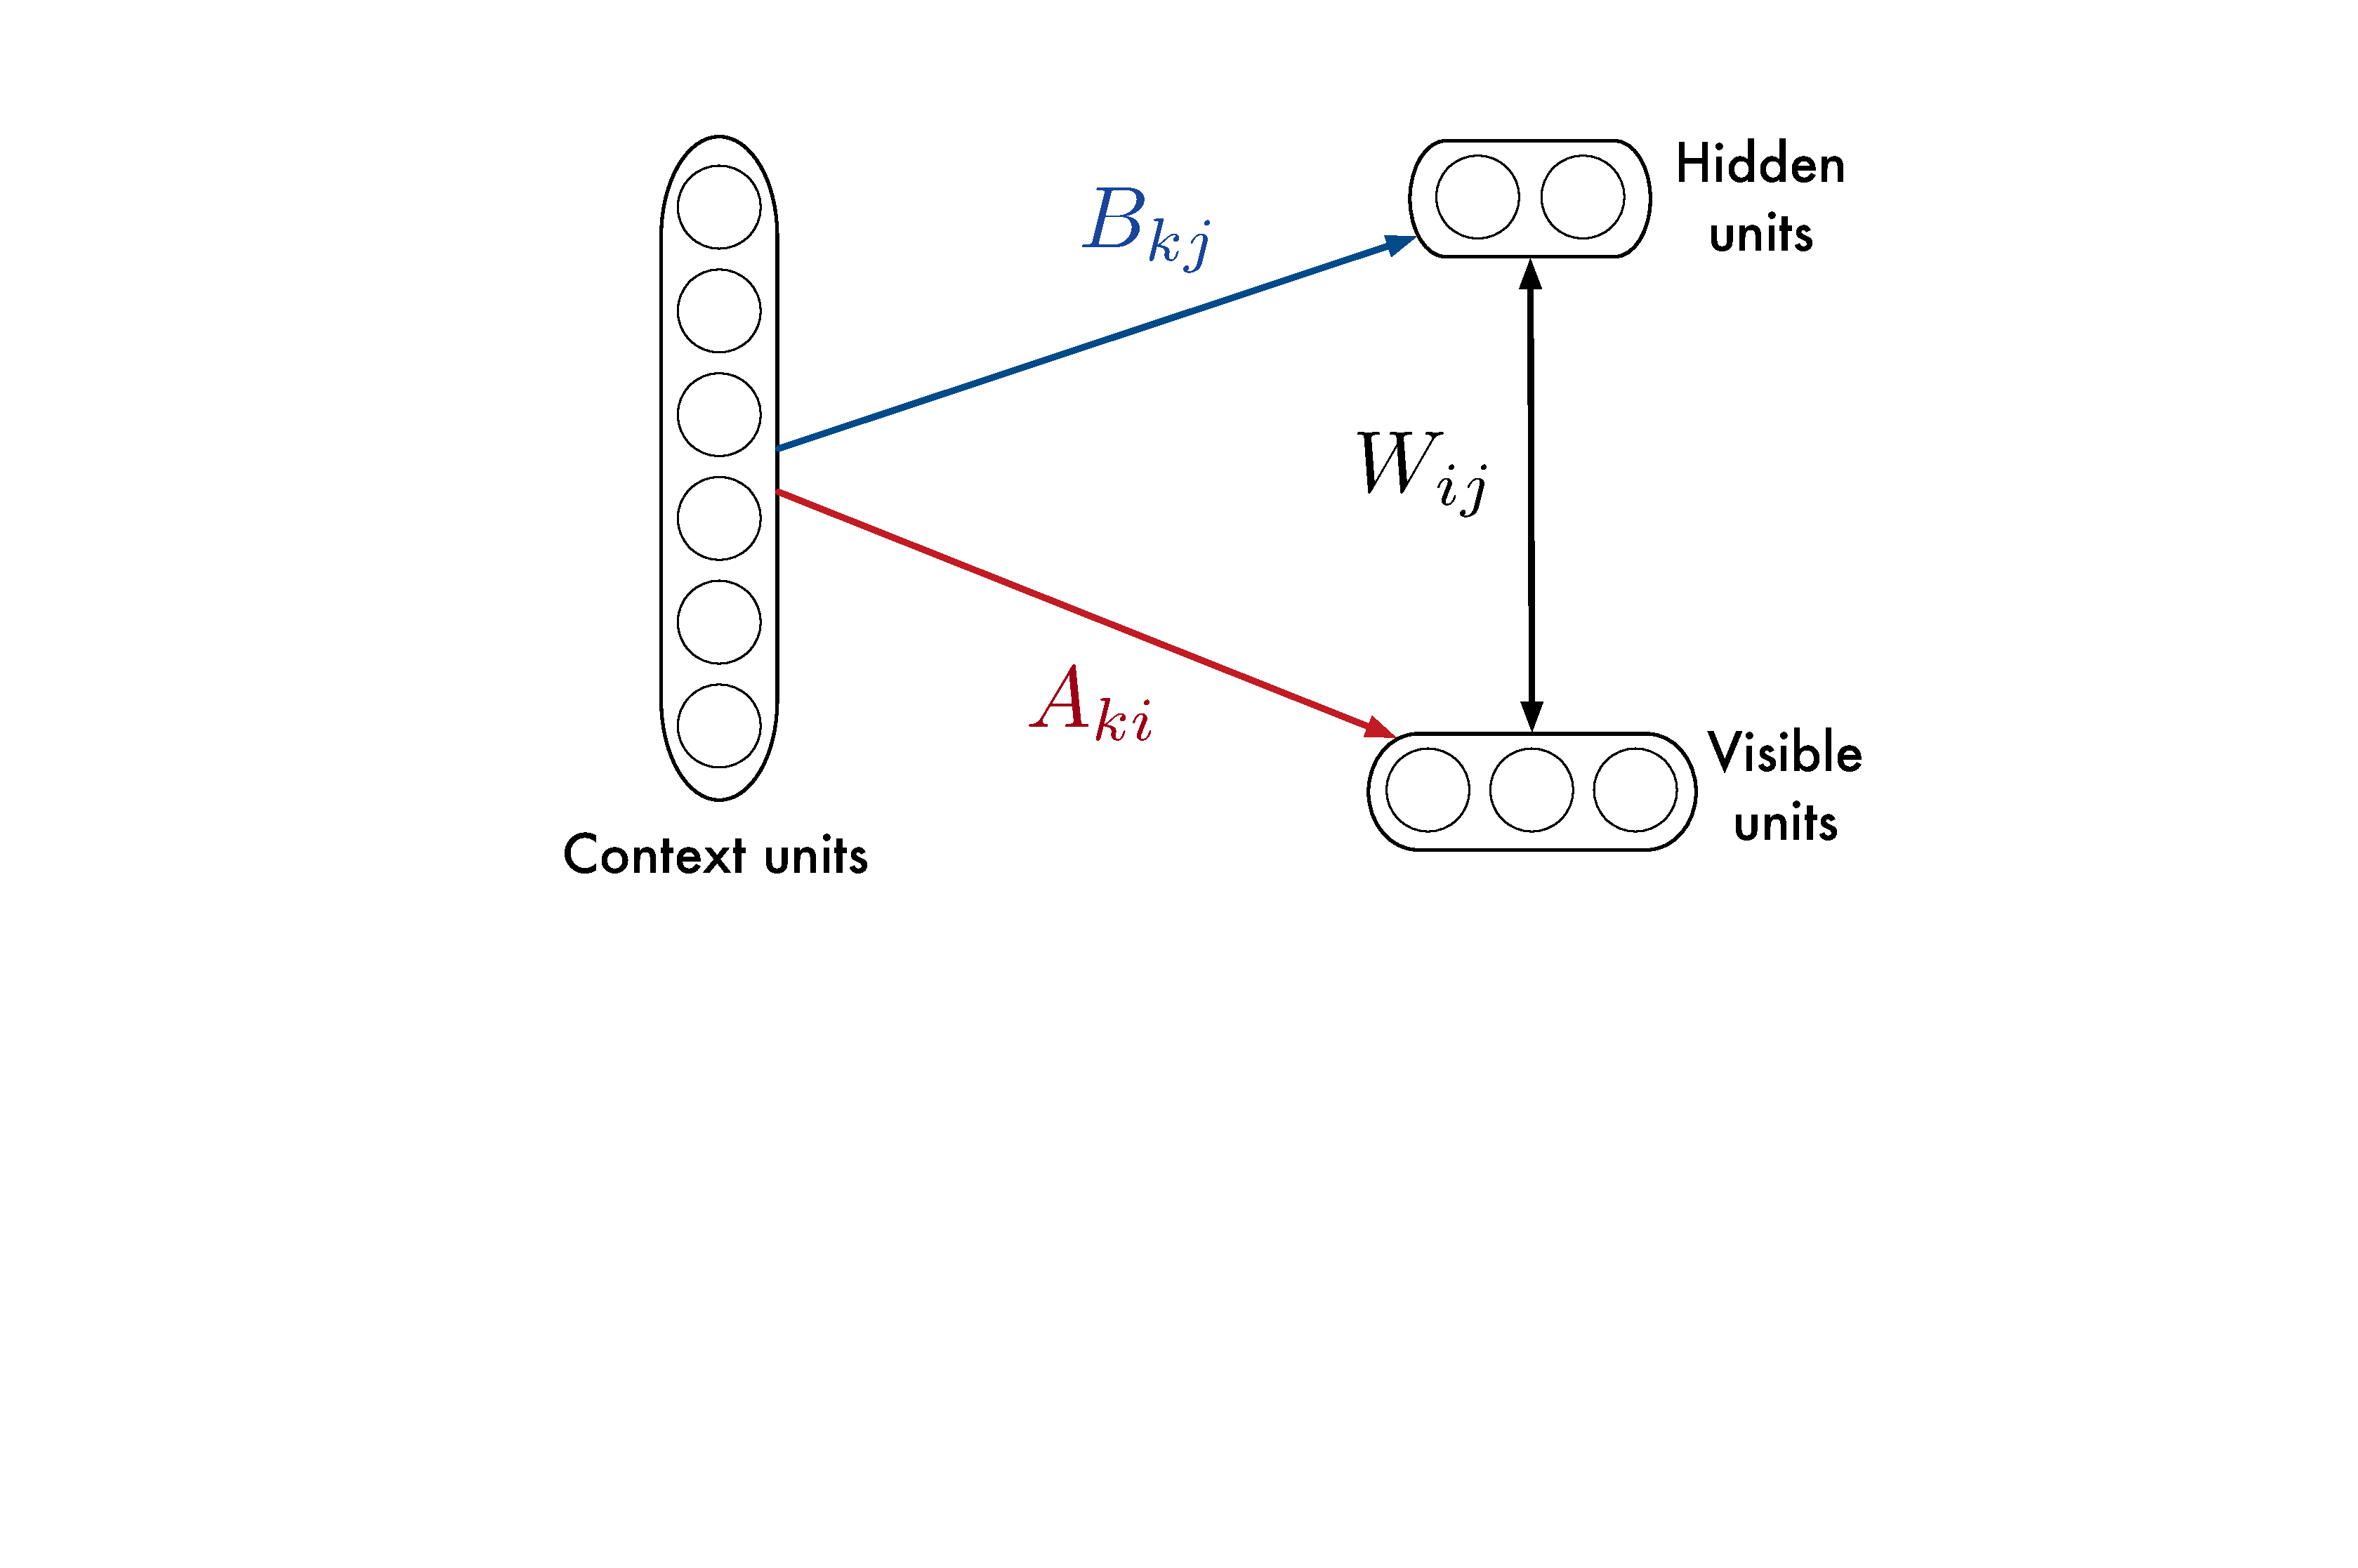
\includegraphics[scale=0.26]{cRBM_orchestration}
\caption{\textit{The conditional RBM} (\textit{cRBM}) adds a layer of context units to the standard RBM architectures. Those context units linearly modify the biases of both visible and hidden units.}
\end{figure}

\subsection{Factored Gated cRBM}
The Factored Gated cRBM model (FGcRBM) \cite{taylor2009factored} proposes to extend the cRBM model by adding a layer of feature units $\bm{z}$ which modulate the weights of the conditional architecture in a multiplicative way. Hence, the parameters of the model become $\bm{\theta} = \left\lbrace \bm{W} , \bm{A} , \bm{B} , \bm{a} , \bm{b} \right\rbrace$, where $\bm{W} = (W)_{ijl}$, $\bm{A}=(A)_{ikl}$ and $\bm{B}=(B)_{jkl}$ are three-dimensional tensors.

This multiplicative influence can be interpreted as a modification of the energy function of the model. For a fixed configuration of feature units, a new energy function is defined by the \textit{cRBM} ($\bm{v}$, $\bm{h}$, and $\bm{x}$). The number of parameters grows cubically with the number of units. To reduce the computation load, the three dimensional tensors can be factorized into a product of three matrices by including factor units indexed by $f$ such that $W_{ijl} = W_{if} . W_{jf} . W_{lf}$.
The energy function of the \textit{FGcRBM} is then given by
\begin{equation}
\begin{split}
E(\bm{v}(t),\bm{h}(t)|\bm{x}(t),\bm{z}(t)) = - \sum_{i} \hat{a}_{i}(t)v_{i}(t) - \\ \sum_{j} \hat{b}_{j}(t)h_{j}(t)
-\sum_{f}\sum_{ijl} W_{if}^{v} W_{jf}^{h} W_{lf}^{z} v_{i}(t) h_{j}(t) z_{l}(t) 
\end{split}
\end{equation}
where the dynamic biases of the visible and hidden units are defined by
\begin{equation}
\hat{a}_{i}(t) = a_{i} + \sum_{m} \sum_{kl}A_{im}^{v}A_{km}^{x}A_{lm}^{z}x_{k}(t)z_{l}(t)
\end{equation}
\begin{equation}
\hat{b}_{j}(t) = b_{j} + \sum_{n} \sum_{kl}B_{jn}^{h}B_{kn}^{x}B_{ln}^{z}x_{k}(t)z_{l}(t)
\end{equation}

\begin{figure}
\centering
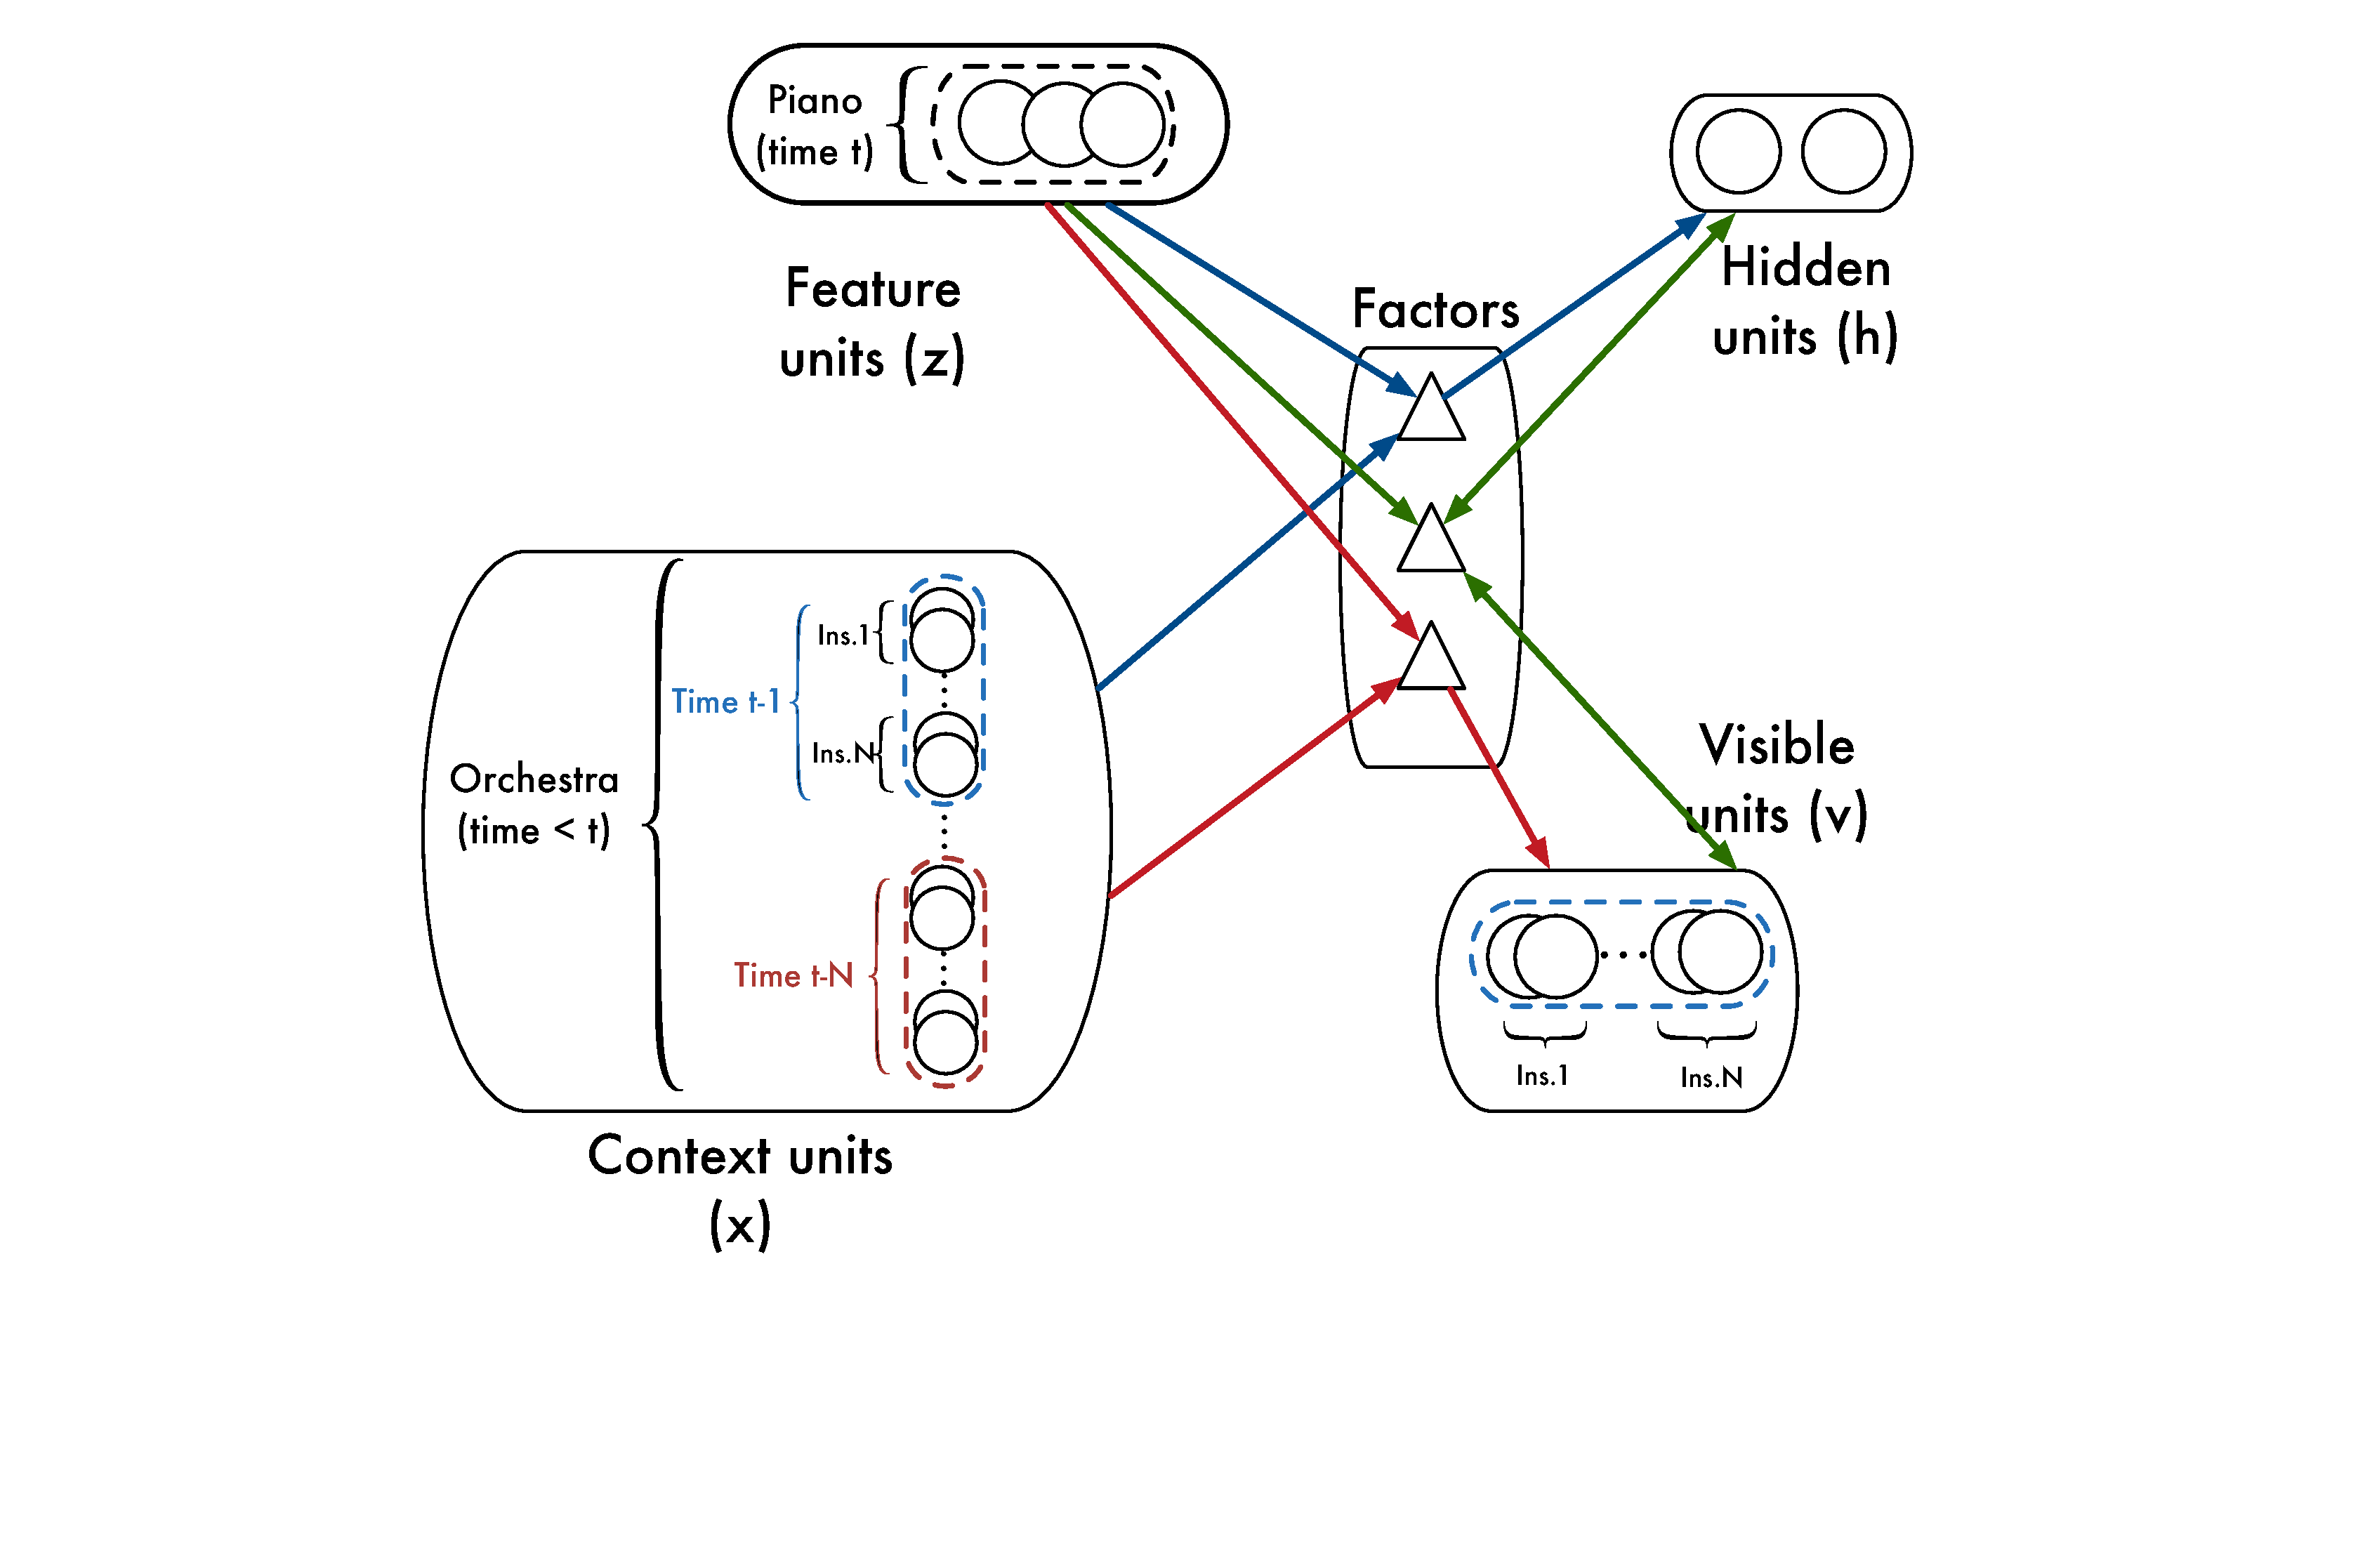
\includegraphics[scale=0.20]{FGcRBM_orchestration}
\caption{\textit{FGcRBM} model. The features units ($\bm{z}$) modify the energy landscape of the model through a multiplicative influence over the weights $\bm{A}$, $\bm{B}$ and $\bm{W}$. Here, the role of each unit in the context of orchestration is indicated.}
\label{fig:FGcRBM}
\end{figure}

%The \textit{FGcRBM} model can be trained by contrastive divergence which lead to the following update rules for the parameter
%\begin{align*}
%\Delta b_{i}^{(v)} &= <v_{i}>_{data} - <v_{i}>_{model}\\
%\Delta b_{j}^{(h)} &= <h_{j} >_{data} - <h_{j} >_{model}\\
%\Delta W_{if}^{v} &= <v_{i}\sum_{j} W_{jf} h_{j} \sum_{l} W_{lf} z_{l}>_{data} - <v_{i}W_{jf} h_{j} \sum_{l} W_{lf} z_{l} >_{model}\\
%\Delta W_{jf}^{h} &= <h_{j}\sum_{i}W_{if}v_{i} \sum_{l} W_{lf} z_{l}>_{data} - <h_{j}\sum_{i}W_{if}v_{i} \sum_{l} W_{lf} z_{l}>_{model}\\
%\Delta W_{lf}^{z} &= <z_{l}\sum_{i}W_{if}v_{i} \sum_{j} W_{jf}h_{j}>_{data} - <z_{l}\sum_{i}W_{if}v_{i} \sum_{j} W_{jf}h_{j}>_{model}\\\Delta A_{im}^{v} &= <v_{i}\sum_{k}A_{km}x_{k} \sum_{l}A_{lm}z_{l}>_{data} - <v_{i}\sum_{k}A_{km}x_{k} \sum_{l}A_{lm}z_{l}>_{model}\\
%\Delta A_{km}^{x} &= <x_{k}\sum_{i}A_{im}v_{i} \sum_{l}A_{lm}z_{l}>_{data} - <x_{k} \sum_{i}A_{im}v_{i} \sum_{l}A_{lm}z_{l}>_{model}\\
%\Delta A_{lm}^{z} &= <z_{l} \sum_{i}A_{im}v_{i} \sum_{k}A_{km}x_{k}>_{data} - <z_{l} \sum_{i}A_{im}v_{i} \sum_{k}A_{km}x_{k}>_{model}\\
%\Delta B_{jn}^{z} &=  <h_{j} \sum_{k}B_{kn}x_{k} \sum_{l}B_{ln}z_{l}>_{data} - <h_{j} \sum_{k}B_{kn}x_{k} \sum_{l}B_{ln}z_{l}>_{model}\\
%\Delta B_{kn}^{z} &= <x_{k} \sum_{j}B_{jn}h_{j} \sum_{l}B_{ln}z_{l}>_{data} - <x_{k} \sum_{j}B_{jn}h_{j} \sum_{l}B_{ln}z_{l}>_{model}\\
%\Delta B_{ln}^{z} &= <z_{l} \sum_{j}B_{jn}h_{j} \sum_{k}B_{kn}x_{k}>_{data} - <z_{l} \sum_{j}B_{jn}h_{j} \sum_{k}B_{kn}x_{k}>_{model}
%\end{align*}

\subsection{Sampling from the models}
% Role des unités conditionelles et tout le tralala dans les modèles
Using gradient descent during the learning phase brings no guarantee about how close of the data distribution the model distribution is. However, the two distribution are supposed to be close (in the sense of the Kullback-Leibler divergence \cite{hinton2002training}) if the training process went fine.
Therefore, by sampling from the model distribution, we are able to generate novel data \textit{similar} to the one observed in the training dataset. 
\textbf{Sampling from a trained model means being able to draw samples from the model distribution marginalized over the visible units $p(v) = \sum_{h} p(v,h)$.}
This remains computationally intractable in the introduced models still because of the partition function. However, samples from an approximate distribution can be reached through alternate Gibbs sampling. After randomly setting the visible units (for each index $i$, $\bm{v}_{i} \sim \mathcal{U}(0,1)$), K Gibbs sampling steps are performed to obtain a visible sample. The objective of these K steps is to reach the equilibrium distribution of the model. Even though a theoretically  infinite number of steps is necessary, 20 to 100 steps are typically sufficient.
Note that, in practice, a threshold is applied on the activation of the visible units before the last sampling step in the \textit{Gibbs chain} so that unlikely activations are simply set to zero.

\begin{figure}
\centering
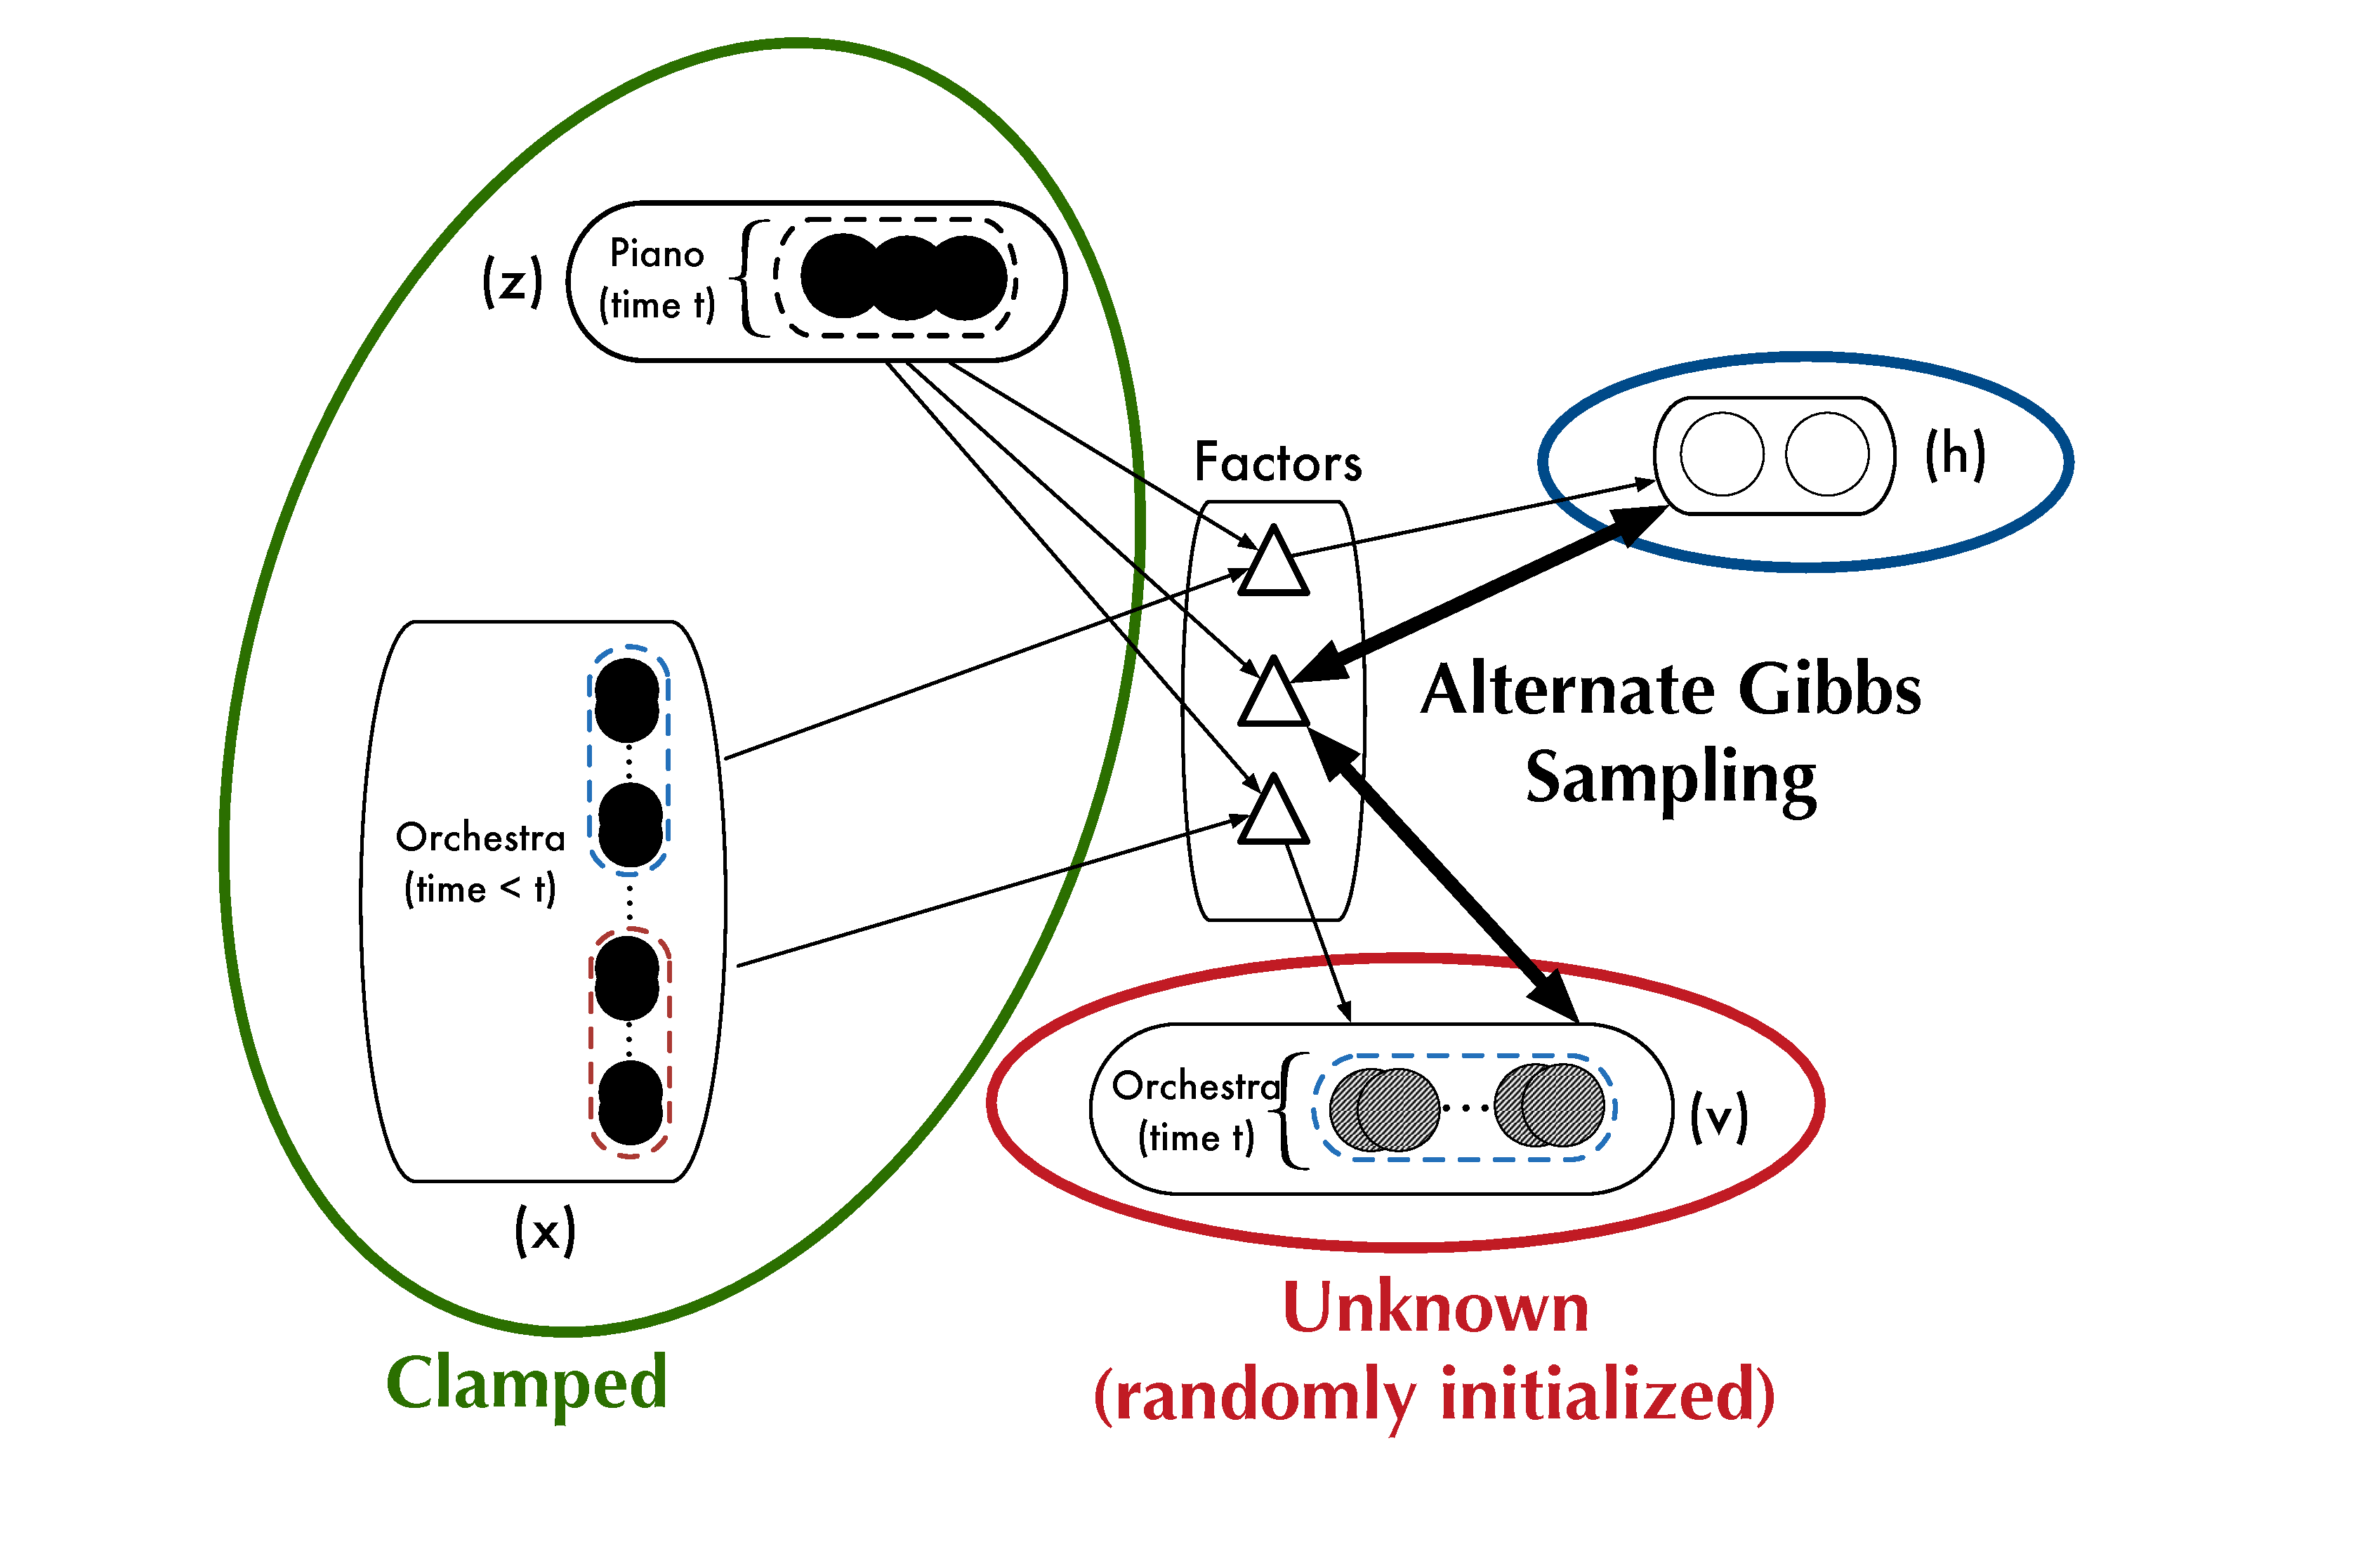
\includegraphics[scale=0.14]{FGcRBM_sampling}
\caption{\textit{Sampling in a FGcRBM}. Context and feature units are respectively clamped to the last ($t-1$ to $t-N$) orchestral frames and the current ($t$) piano frame. Visible units are randomly initialized. Then, several Gibbs sampling step are performed until reaching the equilibrium distribution of the model.}
\label{fig:FGcRBM_sampling}
\end{figure}


\section{Projective orchestration}
In this section, we introduce and formalize the automatic projective orchestration of a piano score as presented in \prettyref{fig:orch}. In particular, we detail the database used, data representation, evaluation framework, and the results obtained by different models in this framework.

\subsection{Database}
We use a database of piano scores and their orchestration by famous composers. The database consists of 76 excerpts of  orchestral pieces, and fourteen different instruments were present in the database.

\subsection{Data representation}
\label{sec:data_representation}
In order to process the score, we represent them as \textit{piano-rolls}, a data representation traditionally used to model polyphonic music of a single instrument (see \prettyref{fig:piano-roll}). The piano and orchestra scores are represented in two different \textit{piano-rolls}. The orchestra \textit{piano-roll} is the concatenation of the \textit{piano-rolls} of each instrument along the pitch dimension.

For a piece of music, we define two multi-dimensional time series $Orch(t)$ and $Piano(t)$ with $t$ in $\left[ | 1 , N_{T} | \right]$ where $N_{T}$ is the lenght of the piece. Those are respectively defined by the sequence of column vector from the \textit{piano-roll} representation of the orchestra part and of the piano part.

At each time frame $t$, the visible units of the cRBM represent the current orchestral vector ($Orch(t)$) that we want to generate. Conditional units are used to model the influence of the past orchestral vectors $Orch(t-1) , ... , Orch(t-N)$ and the influence of the current piano frame ($Piano(t)$) over the visible units. Hence, in the \textit{cRBM} model, the context units at time $t$, $\bm{x}(t)$, are defined by the concatenation of the past orchestral frames and current piano frame
\begin{equation}
\bm{x}(t) = \left[ \text{Piano}(t) , \text{Orch}(t-1) , ... , \text{Orch}(t-N)\right]
\end{equation}

The \textit{FGcRBM} model allows to separate the influence of the current piano frame and the past orchestral frames. Hence, the current piano frame defines the feature units $\bm{z}(t)$ 
\begin{equation}
\bm{z}(t) = \text{Piano}(t)^{T}
\end{equation}
while the concatenation of the past orchestral frames defines the context units $\bm{x}(t)$
\begin{equation}
\bm{x}(t) = \left[ \text{Orch}(t-1)^{T} , ... , \text{Orch}(t-N)^{T} \right]^{T}
\end{equation}

\begin{figure}
\centering
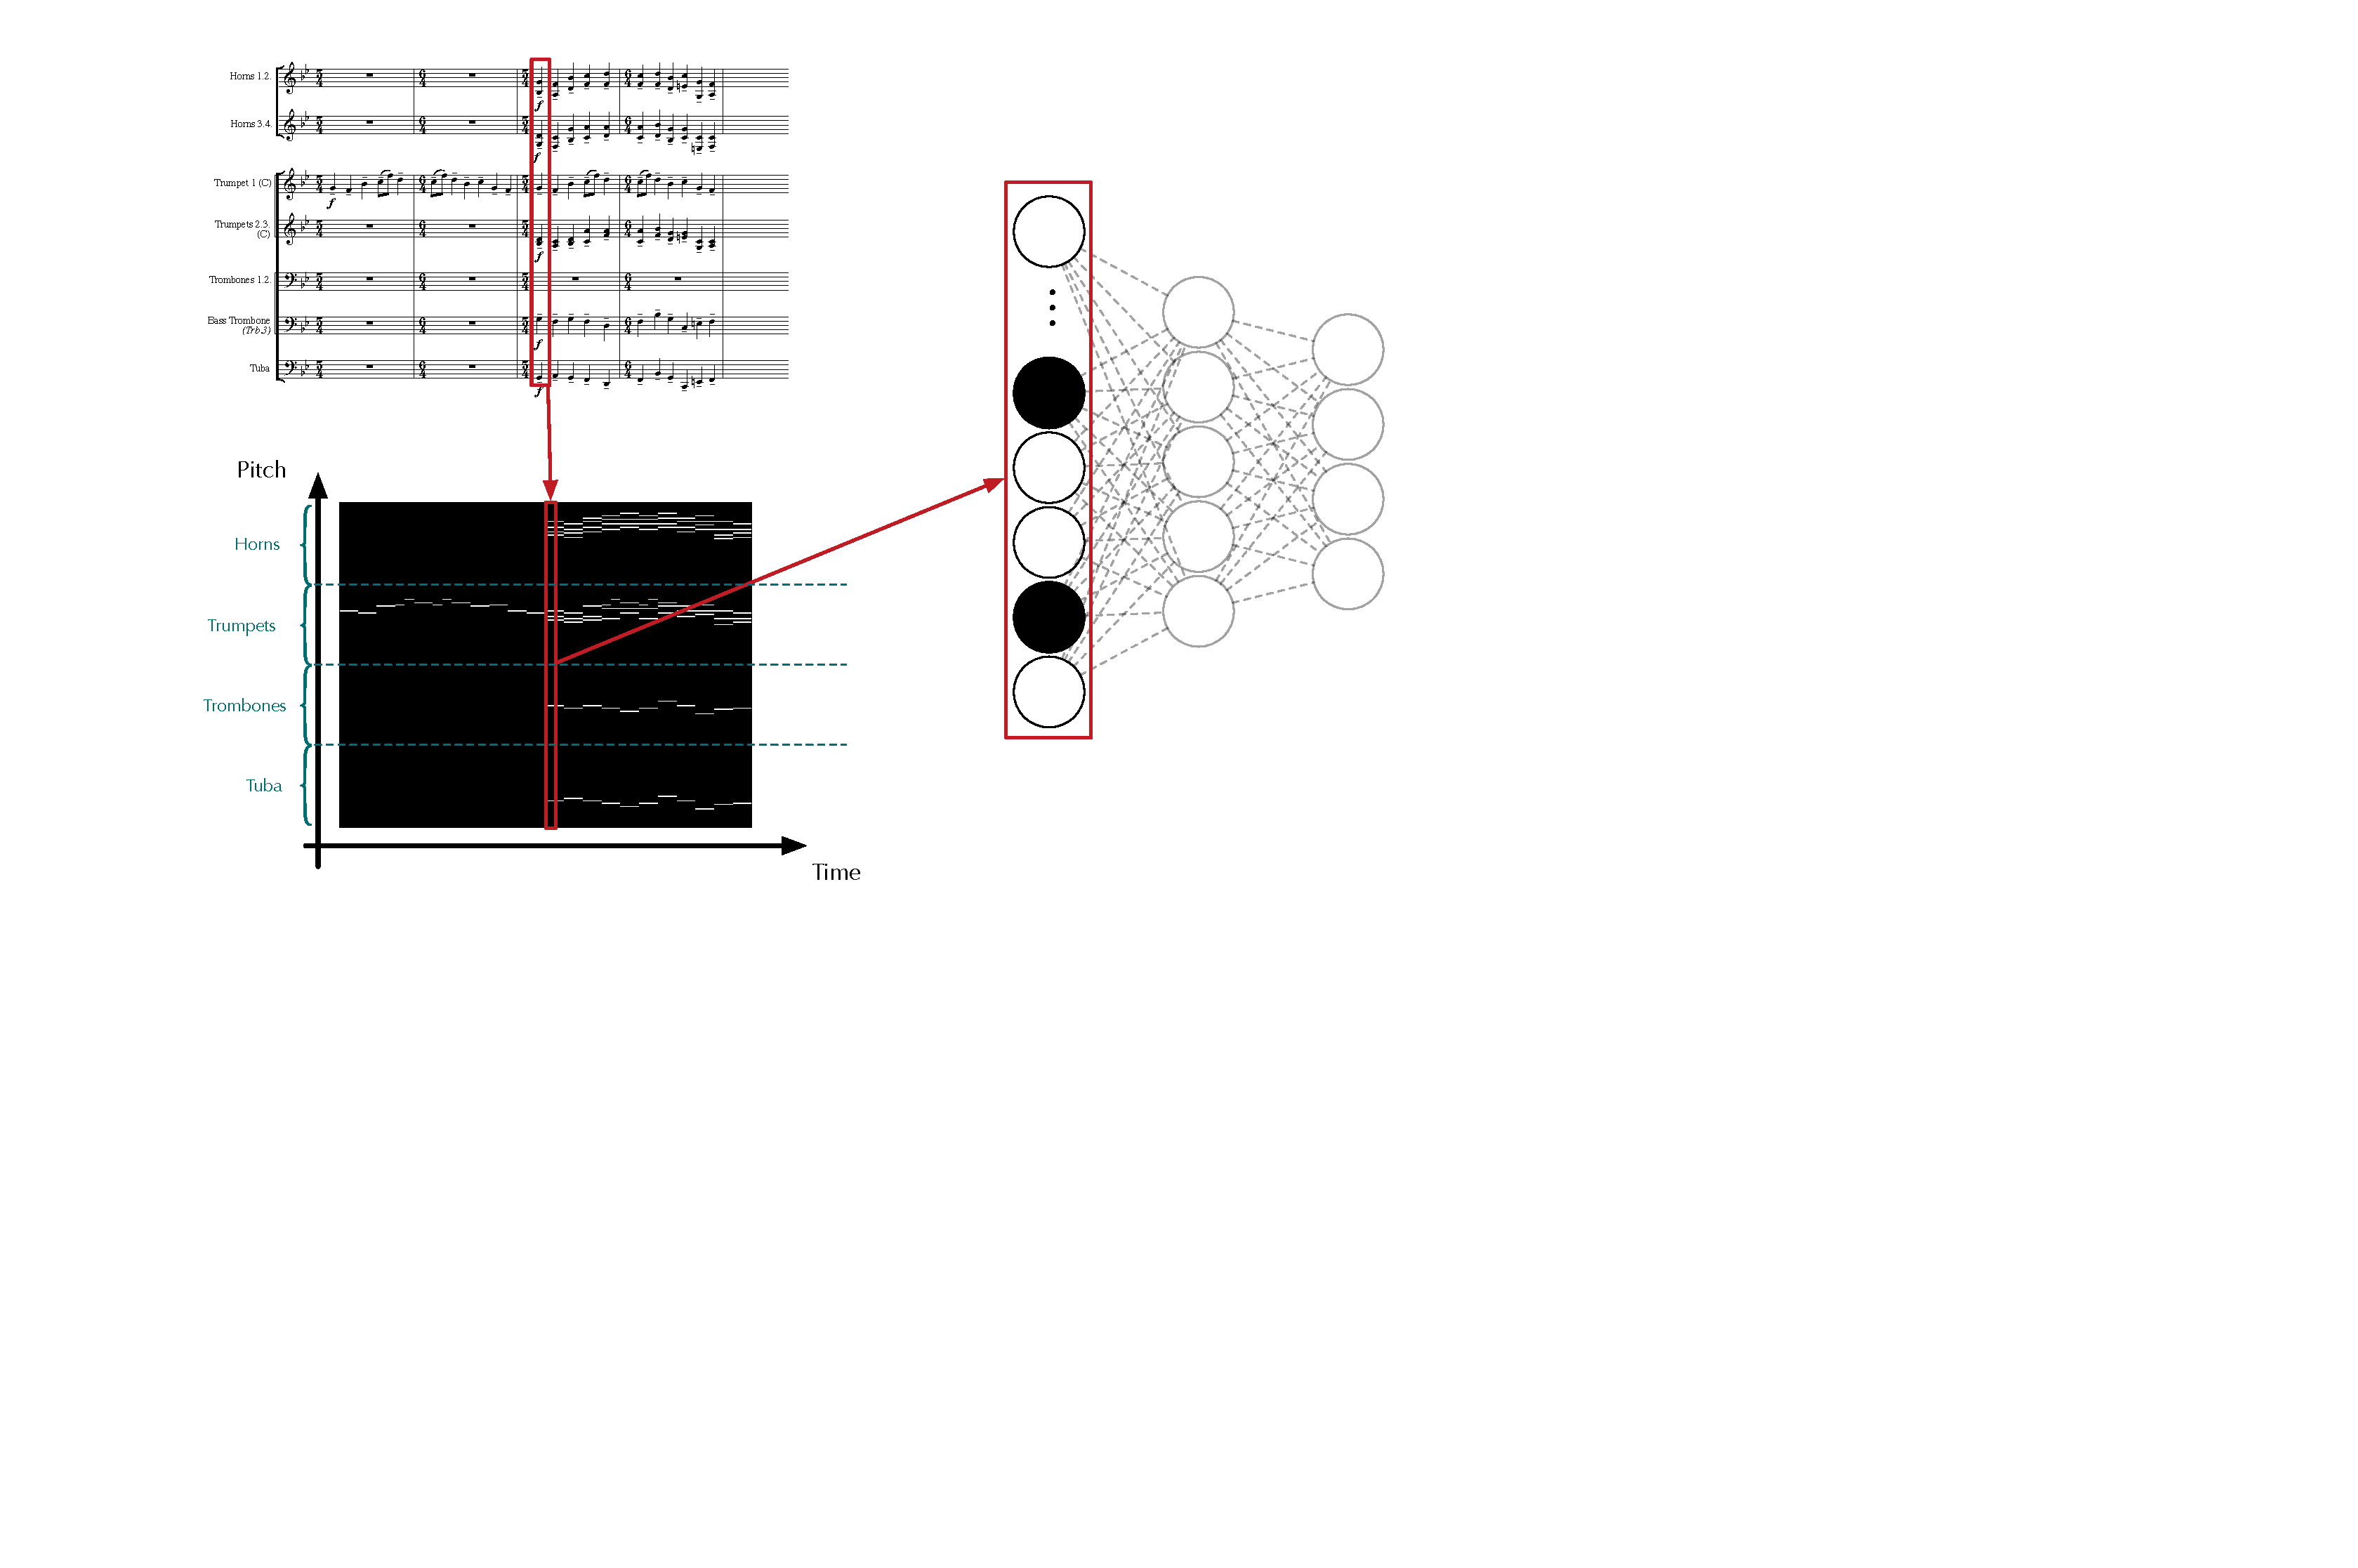
\includegraphics[scale=0.35]{data_representation}
\caption{The successive visible units of a neural network could be the successive temporal frames of a \textit{piano-roll}. A \textit{piano-roll} is a representation of musical events, discrete on both the frequency (pitch) and the time (frames) scales. For a single instrument, a pitch $p$ at time $t$ can be either played or not, which is represented by a one or zero in the \textit{piano-roll}. This definition is extended to an orchestra by simply concatenating the \textit{piano-rolls} of each instruments along the pitch dimension. One can see on the figure that the same instruments are grouped together event if they don't play the same thing. For instance, trumpets 1, 2, 3 and 4 are grouped under one trumpet part, which then contains 4 voices chords.}
\label{fig:piano-roll}
\end{figure}

\subsection{Evaluation framework}
We process the score with a rhythmic quantization, the number of time frame in the \textit{piano-roll} per quarter note, of 8.
The velocity information is lost, since we use binaries units which solely indicates if a note is on or off. 

In order to reduce the number of units we systematically remove, for each instrument, any pitch which is absent from the training database. Hence, the dimension of the orchestral vector decreased from 2432 to 191 and the piano's one from 128 to 43.
Also, we follow the classic orchestral simplifications used when writing orchestral scores by grouping together all the instruments of a same section. For instance, the \textit{violin} section, composed by many instrumentalists (10 or more), is written as a single part.

Data used to evaluate the performance of the models can not be the same as the one used to train it. The data set is usually split between a train and test set \cite{bishop2006pattern}.
Given the complexity of the distribution we wanted to model and the extremely narrow size of the database, 75 and a half files were used to train the model a half file for testing. This choice is motivated by the will to obtain the best generative model possible.

\label{sec:event-level}
We propose to work in an \textit{event-level} framework, instead of a traditional \textit{frame-level} \cite{DBLP:journals/corr/YaoCVDD15,boulanger2012modeling,lavrenko2003polyphonic}. In a frame-event level framework, each time frame is a training point. 
In an event-level framework, training point are only those for which an \textit{event} occurs. An event occurs at time $t_{e}$ when $\text{Orch}(t_{e}-1) \neq \text{Orch}(t_{e})$. Test points will also be selected among new event time indices. The reason why we don't train and evaluate on each frame is that in a \textit{frame-level} framework a model which simply repeats the previous frame gradually becomes the best model as the quantization increases. Moreover, in the projective orchestration framework, rhythmic patterns is established by the known piano score or input, and thus, does not have to learned by the model.

% Nombre de batch
Finally, to speed-up the convergence of the gradient descent, mini-batches are used to train the model \cite{bishop2006pattern}. 89 mini-batches of 100 event-level points were obtained.

%% DAta pas shuffled entre train et test, justifier pourquoi

\subsection{Measure}
An objective criterion of the performance of a model is necessary to provide our evaluation. 
The best way for evaluating generative models is to compute the likelihood (\prettyref{eq:likelihood}) of the test set. However, we have seen that this quantity is intractable in a \textit{RBM}, \textit{cRBM} or \textit{FGcRBM} (\prettyref{eq:likelihood}).

A solution is to define an auxiliary evaluation task. A task commonly used in the closely related field of automatic music generation is a short-term predictive task based on a frame-level accuracy measure \cite{DBLP:journals/corr/YaoCVDD15,boulanger2012modeling,lavrenko2003polyphonic}. Based on this framework, we introduce an \textit{event-level orchestral inference} task to evaluate our models. To our best knowledge, this is the first attempt to define a quantitative evaluation framework for automatic projective orchestration.

The task consists in comparing the prediction of the model with ground-truth orchestration from a test dataset of existing orchestration proposed by experts (composers). More precisely, for an \textit{event} $t_{e}$ (see \prettyref{sec:event-level}), the visible units of the model are sampled with its context units set to $Piano(t_{e})$ and $Orch(t_{e}-1),... Orch(t_{e}-N)$ from the test dataset. This sampled prediction, denoted $\hat{\text{Orch}}(t_{e})$, is then compared to the ground-truth vector $\text{Orch}(t_{e})$ from the test dataset via the accuracy measure
\begin{equation}
\text{Accuracy}  = \frac{TP(t)}{TP(t) + FP(t) + FN(t)}
\label{eq:accuracy}
\end{equation}
where $TP(t)$ (true positives) is the number of notes correctly predicted (note played in the prediction and ground-truth). $FP(t)$ (false positive) is the number of notes predicted which are not in the original sequence (note played in the prediction, but not in ground-truth). $FN(t)$ (false negative) is the number on unreported notes (note absent in prediction, but played in ground-truth). 
Instead of binary values, activation probabilities are used for the predicted samples in order to reduce the sampling noise.

\begin{figure}
\centering
\begin{tabular}{c c}
\hline
Model & Orchestral Event-level (\%)\\
\hline
Random & 0.50\\ 
\hline \hline
cRBM & 1.5\\ 
FGcRBM & 2.2\\ 
\end{tabular}
\caption{Event-level accuracy for the orchestral inference task.}
\label{fig:result_event_level}
\end{figure}

\subsection{Results}
The results are given in \prettyref{fig:result_event_level}. The random model is a Bernouilli distribution of parameter $0.5$.

The results of the random distribution are lower than the cRBM and FGcRBM models. The FGcRBM have better results than the cRBM model, which suggests that the separation between features and context improves the model.
However, the results are relatively bad, and the we observe that the activation probability of the visible units during the generation process is unexpectedly noisy (FIGURE). We believe that those models are actually not adapted to the sparse binaries data we try to model. Indeed, the auto-correlation matrices would be more adapted to model continuous data.

%\begin{figure}
%\centering
%\begin{tabular}{c c}
%\hline
%\multirow{2}{*}{Model} & \multicolumn{1}{c}{Frame Acc \%} \\
%\hhline{~-}
%& JSB Chorales\\
%\hline
%Random & 4.22\\ 
%Repeat & 39.60\\
%Random fields & \textcolor{green}{\textbf{22.93}}\\ 
%LSTM with Rprop & \textcolor{orange}{\textbf{31.91}}\\ 
%RNN-RBM & \textcolor{orange}{\textbf{33.12}}\\ 
%\hline \hline
%Temporal RBM & \textbf{30.52}\\ 
%cRBM &  \textbf{31.18}\\
%HcRBM & - \\ 
%\end{tabular}
%\caption{Frame level accuracy for polyphonic music. Evaluated on JSB chorales database. Results of other models are from \cite{boulanger2012modeling}}
%\label{fig:result_frame_level}
%\end{figure}

\subsection{Discussion : evaluating a generative model ?}
It is important to state that we don't consider this predictive measure as as reliable measure of the creative performance of a model. Indeed, predicting and creating are two fairly different things. However, we believe that for basic generative models, the \textit{best} one would be the one which managed to grasp most of the structure in the training database. From this point of view, apredictive measure can be acceptable for model selection purposes.

This measure then allow us to select the best model (a \textit{FGcRBM}) and its optimal set of hyper-parameter. We then implemented the trained network in a generative real-time framework introduced in the next section.

\section{Live Orchestral Piano (LOP)}
We introduce in this section the \emph{Live Orchestral Piano} (LOP)
application, which is the first software able to provide a way to
compose music with a full classical orchestra in real-time by simply
playing on a MIDI piano. The goal of this framework is to rely on
the knowledge learned by the model introduced in the previous sections
in order to perform the projection from a piano melody to the orchestra.

\subsection{Workflow}
The software is implemented on a client/server paradigm. This choice
allows to separate the orchestral computation part from the interface
and sound rendering engine. That way, multiple interfaces can easily
be implemented. It should also be noted that separating the computing
and rendering on different computers, can allow to use high-quality
and CPU-intensive orchestral rendering plugins. This can allow a more
realistic orchestral rendering with heavy amounts of computation performed
while ensuring the real-time constraint on the overall system (preventing
degradation of the computing part). The complete implementation workflow
is presented in Figure~\ref{fig:Live-orchestral-piano}.

\begin{figure*}
\begin{centering}
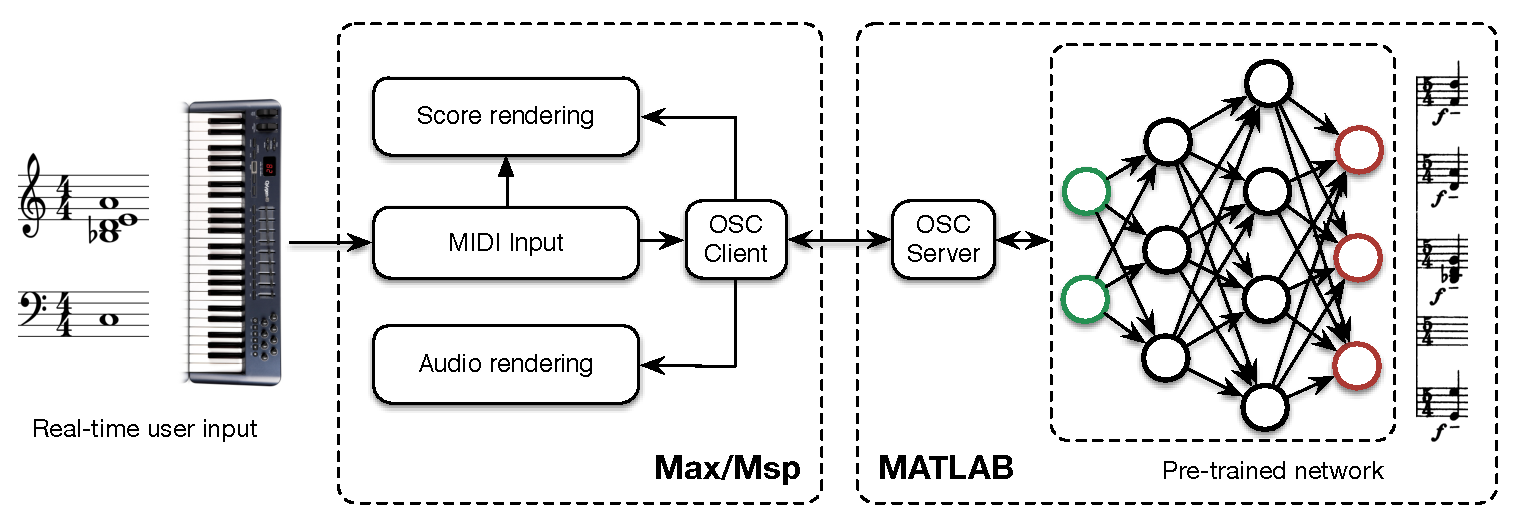
\includegraphics[scale=0.55]{workflow}
\par\end{centering}

\caption{\label{fig:Live-orchestral-piano}Live orchestral piano (L.O.P) implementation
workflow. The user inputs a melody which is transcribed into a score
and send via OSC from the Max/Msp client. Then, the MATLAB server
uses this vector of notes and process it following the aforementioned
techniques in order to obtain the orchestration. This information
is then sent back to Max/Msp which performs the real-time audio rendering }
\end{figure*}


As we can see, the user can input a melody (single notes or chords)
through a MIDI keyboard, which is retrieved inside the Max/Msp interface.
The interface transmits this symbolic information (as a variable-length
vector of active notes) via OSC to the MATLAB server. The interface
performs a real-time transcription of the piano score to the screen
in parallel. The server uses this vector of events to produce an 88
vector of binary input note activations (as defined in Section~\textbf{XXX}).
This vector is then processed by using the orchestration algorithms
presented in Section~\textbf{XXX} in order to obtain a projection
of a specific symbolic piano melody to the full orchestra (an operation
defined as \emph{projective orchestration}). The resulting orchestration
is then sent back to the client interface which performs both the
real-time audio rendering and score transcription. 

\textbf{NB: A good thing would be to compute the end-to-end latency
in the system ! And also to compute this with a variable number of
Gibbs steps ... all of this to show that we respect real-time constraints
/ requirements.}

\subsection{Interface}
The interface has been developed in Max/Msp, to facilitate both the
score and audio rendering aspects in a real-time environment. The
score rendering is handled by the \emph{Bach }library environment
\textbf{{[}INSERT REF{]}}. This interface provides a way to easily
switch between different orchestration models, while controling other
meta-parameters of the sampling. For instance the \emph{cutoff probability
}gives a direct access to the density of the generated orchestration
(in terms of number of played instruments). Indeed, a low cutoff probability
implies that most activation of notes will be taken into account in
the playback, while a high cutoff will produce more sparse orchestration.

\textbf{{[}INCLUDE FIGURE WITH LIVE EXAMPLE{]}}

\subsection{Examples}

Score and videos ?


\subsection{Offline generation}

Retry to generate full orchestral scores from piano scores. (with
new threshold and unit-variance transform) 

+ Assess various thresholds of generation

+ Try on Moussorgski and Beethoven


%\section{Live Orchestral Piano}

\section{Conclusion and future works}
% Interesting and highly benefit problem
The general objective of building a generative model for time series is one of the most prominent topic of interest for the machine learning field. Orchestral inference sets a slightly more specific framework where the generated time series is conditioned by an other observed time series (the piano). It is a challenging and worthwhile task and tackle it would benefit the machine learning field in many aspect.

% Increase DB
The high dimensionality of the data and their sparsity are a major obstacle for learning algorithms.
A first remark is that a larger database would be required to train any model sufficiently complex to properly represent \textit{THIS} distribution.
It is important to build a clean reference database of piano scores and their orchestration. By clean we mean with an good orchestration (by acknowledge composers), with all instrument name indicated and velocity for the notes. 

% Change the data representation 
% Velocities
Indeed, we believe that taking the notes' velocity into consideration is crucial, since many orchestral effects are justified by intensity variations in the original piano scores. 
% Find distrib representations
Besides, the sparse representation of the data suggests that a more compact distributed representation might be found. Lowering the dimensionality of the data would greatly improve the efficiency of the learning procedure. For instance, methods close to the word-embedding techniques used in natural language processing might be useful \cite{kiros2015skip}. 
% Time dimension :
% 1 - Several granularity
% 2 - Frame-level -> pbm quantization
Along the time dimension, two remarks about \textit{temporal granularity} and \textit{time quantization} should be made. A piece of music is structured by different range of temporal dependencies. For instance, we can roughly distinguish short-term, from the previous note over the next one, mid-term, inside a bar, and long-term (theme, development and re-exposition of the theme) dependencies that we referred to as different temporal granularity. We believe that a model which would include different temporal dependencies would generate more coherent orchestrations.
The rhythmic structure of the piano score is an other important structural dimension that has been discarded in our system. Indeed, by working with an event-level temporal granularity, the rhythmic information is lost. However, slow and fast movements will not be orchestrated in the same fashion. Thus, it is necessary to preserve this information by considering the series formed by all the successive frames of the piano-roll, \textit{i.e.} a frame-level quantization. Several problem arise when working in a frame-level quantization, the first one being to chose the size of the frame.
% Multi-modal
Finally, a more ambitious improvement would be to add audio data to the symbolic information of the score. Indeed, we believe that despite \textit{EN GROS LA ON DIT QUE L'HYPOTHESE DU DEPART (KNOWLEDGE COMPOSERS ABOUT TIMBRE EMBEDDED IN SCORE) CEST DE LA MERDE...}.

% Increase baseline
Besides these modifications on the nature of the processed data, a lot of models already existing could be easily adapted to the particular problem of orchestral inference and should be evaluated to form a solid baseline.
% Measure ?
Secondly, a better performance measure should be developed for the orchestral inference task. A good solution would be to derive estimators for the likelihood of existing sequences under the proposed models.

% Acknowledgmentsinclude

% Bibliography
\bibliographystyle{iccc}
\bibliography{../Biblio/biblio}

\end{document}
